\section{Auswertung}
\label{sec:Auswertung}
\subsection{Funktionengenerator}
Zunächst wird das Signal des Funktionengenerators auf dem Oziloskop ausgegeben. Dort wird die Frequenz der gewählten Sinusfunktion auf 1$\,$kHz justiert und eine Spannung von $52 \cdot 10^{-3}$ Volt gewählt. Anschließend wird der Aufbau wie in der Beschreibung beschrieben aufgebaut. Dabei werden die Filter der Frequenz entsprechend auf 1 Kiloherz angepasst und die Vorerstärkung am Low-Pass Amplifier auf 200 eingestellt. Der Noise Generatoir wird zunächst einmal überbrückt indem er auf off gestellt wird.
\subsection{Phasenabhängigkeit der Ausgangsspannung}
Ziel des Versuchsteil ist es die Abhängigkeit der Ausgangsspannung $U_{\text{out}}$ von der Phasendifferenz $\phi$ der Eingangsspannung $U_{\text{sig}}$ und der Referenzsspannung $U_{\text{ref}}$ genauer zu beobachten. Zunächst wird eine Art offset Messung der Phasenverschiebung der beiden Spannungen durchgeführt. Dafür wird der Phasenwinkel solange justiert bis ein Osziloskopausschlag wie in Bild \ref{fig:phi0} erscheint, was einen Phasenwinkel von $\phi = 0$ entspricht.
\begin{figure}
  \centering
  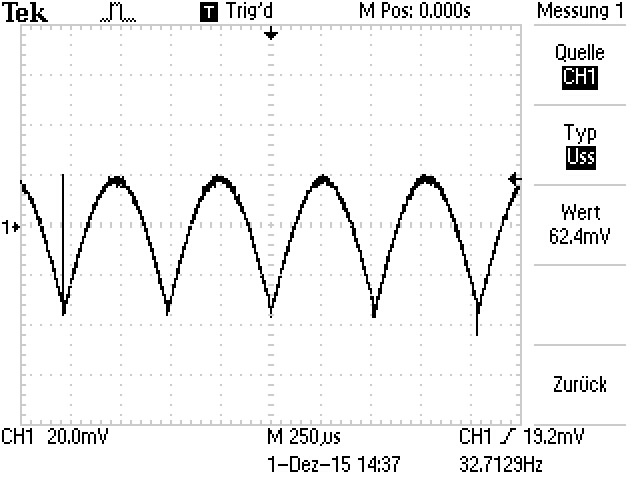
\includegraphics[height=5cm]{picture/1.JPG}
  \caption{$\phi = 0$ , offset Messung.}
  \label{fig:phi0}
\end{figure}
Daran wird die Phasenskala für den weiteren Versuchsverlauf dran ausgerichtet. Mittels eines Tiefpasses wird die Spannung, durch den Innenwiederstand integriert und die Zeitlich gemittelte Spannung auf einem Messgerät ausgegeben. Nach Berücksichtigung der Verstärkung ergibt sich nach Formel \ref{eqn:Uout} für eine Phasenverschiebung von $\phi = 0^{\circ}$ eine Spannung von
\begin{equation}
  U_{\text{out}} = \frac{2}{\pi} \cdot \frac{52 \cdot 10^{-3} \, V}{200} = 33.1 \cdot 10^{-3} \, V
  \label{eqn:Uout}
\end{equation}
Nach Formel ?? werden die theoretischen und praktischen Spannungswerte ausgerechnet und in Tabelle ?? mit dem dazugehörigen Phasenwinkel aufgelistet.
\begin{table}
  \centering
  \begin{tabular}{c c c}
    \toprule
    $\phi$ & $U_{\text{theoretisch}} / 10^{-3} \cdot $ V & $U_{\text{praktisch}} / 10^{-3} \cdot $ V \\
    \midrule
    0	&  33.1  &  32.5	\\
    30	&  28.6  &  27.5	\\
    60	&  16.5  &  12.5	\\
    90	&  0.0 	 &   2.5	\\
    120	& -16.5  & -17.5	\\
    150	& -28.6  & -30.0	\\
    180	& -33.1  & -35.0	\\
    210	& -28.6  & -27.5	\\
    240	& -16.5  & -12.5	\\
    270	&  0.0 	 &  2.5	 	\\
    300	&  16.5  &  17.5	\\
    330	&  28.6	 &  30.0	\\
  \end{tabular}
  \caption{$U_{\text{out}}$ bei verschiedenen Phasen.}
  \label{tab:Uphase}
\end{table}
Abbildung \ref{fig:Spannungsverlauf} kann man entnehmen das die Gemessene Spannung qualitativ erfüllt.
\begin{figure}
  \centering
  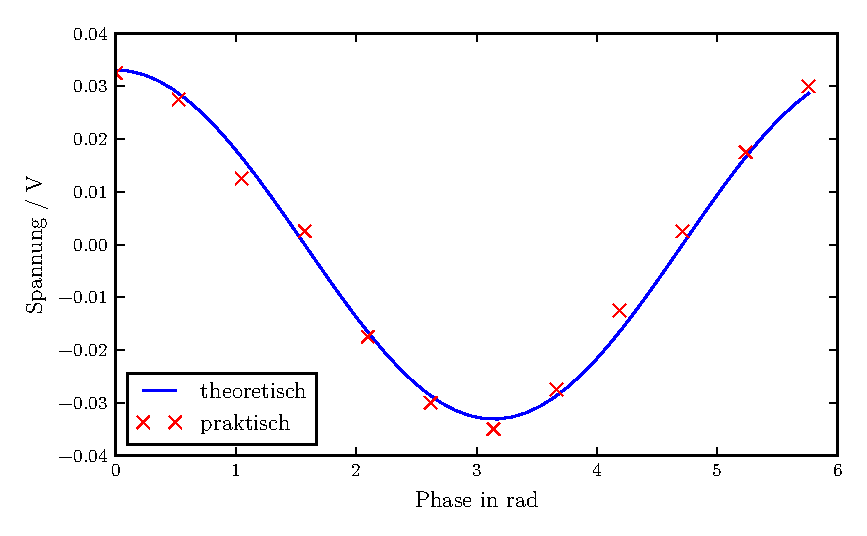
\includegraphics[height=5cm]{Spannungsverlauf.pdf}
  \caption{Spannungsverlauf}
  \label{fig:Spannungsverlauf}
\end{figure}

